\documentclass[compress]{beamer}
\usetheme{Warsaw}
\usecolortheme{crane}
\usepackage[utf8]{inputenc}
\usepackage[portuguese]{babel}
\usepackage{url}
\usepackage{tikz}
\usepackage{color}
\usetikzlibrary{arrows}
\usetikzlibrary{arrows}
\usepackage{default}
\usepackage{amsmath}
\usepackage{amsfonts}
\usepackage{amssymb}
\usepackage{newalg}

% Algumas definições %%%
\def\term#1{{\sc #1}}   % IR terms in examples not index terms!
\def\query#1{{\sf #1}}
\def\oper#1{{\sc #1}} % AND, OR, NOT
%%%%%%%%%%%%%%%%%%%%%%%%

\title[Coelho: Dicionários e Recuperação Tolerante]
{Introdução à Recuperação de Informações\\
\large \url{https://github.com/fccoelho/curso-IRI}\\[0.5cm]
IRI 3: Dicionários e Recuperação Tolerante}

\author [Coelho F.C. \& Souza R.R.]{ Flávio Codeço Coelho}

\institute [EMAp, FGV]{Escola de Matemática Aplicada,   Fundação Getúlio Vargas}
\date


\begin{document}

\begin{frame}
\titlepage
\end{frame}

\begin{frame} %%%%%%%%%%%%%%%%%%%%%%%%%%%%%%
\frametitle{Sumário}
  \tableofcontents
\end{frame}

\section{Recapitulação}

\begin{frame}
\frametitle{Distinguindo entre Tipo e token}
\begin{itemize}
\item {\color{blue}Token} -- Uma instância de uma palavra ou termo ocorrendo 
em um documento
\item {\color{blue}Tipo} -- Uma classe de equivalência de tokens
\item \emph{In June, the dog likes to chase the cat in the barn.}
\item 12 tokens, 9 tipos de palavras
\end{itemize}
% $$L(x) = 1\cdot\frac{x - 2} {1 - 2}\cdot{\frac{x - 3}{1 - 3}}+{4}\cdot{\frac{x 
% - 1}{2 - 1}}\cdot{{x - 3}{2 - 3}}+{9}\cdot{\frac{x - 1}{3 - 1}}\cdot{\frac{x - 
% 2}{3 - 2}}$$
\end{frame}

\begin{frame}
\frametitle{Problemas na tokenização}
\begin{itemize}
\item Quais são os delimitadores? Espaços? Apóstrofes? 
Hífen? 
\item Para cada um destes: às vezes eles delimitam, às vezes não.
\item Muitas línguas não possuem espaços! (P.ex.,
Chinês)
\item Não Há espaços em palavras compostas em Holandês, Alemão e Sueco
(\emph{Lebensversicherungsgesellschaftsangestellter})
\end{itemize}
\end{frame}


\begin{frame}
\frametitle{Problemas com classes de equivalência}
\begin{itemize}
\item Um termo é uma classe de equivalência de tokens.
\item Como definir Classes de equivalência?
\item Números: (3/20/91 vs.\ 20/3/91)
\item Capitalização
\item Truncagem, Truncador de Porter 
\item Análise Morfológica : infleccional vs.\ derivacional
\item Problemas de classes de equivalências em outras línguas
\begin{itemize}
\item Morfologias mais complexas do que o inglês
\item Finlandês: Um único verbo pode ter 12000 formas diferentes
\item Acentos, tremas, etc.
\end{itemize}
\end{itemize}
\end{frame}

\begin{frame}[label=takeaway]
%\begin{frame}
\frametitle{Principais conclusões de hoje}

\begin{itemize}

\pause[2]

\item \myblue{Recuperação Tolerante:} O que fazer se não há correspondência 
exata entre o termo de consulta e os termos do documento.

\pause[3]

\item Consultas coringas

\pause[4]

\item Correção ortográficas

\end{itemize}

\end{frame}

\section{Dicionários}

\begin{frame}
\frametitle{Índice invertido}

Para cada termo $t$, armazenamos uma lista de documentos que contém $t$.

\bigskip

\begin{tabular}{|c|c|r|r|r|r|r|r|r|r|r|}
\cline{1-1}\cline{3-10}
\term{Brutus} & $\longrightarrow$ & 1 & 2 & 4 & 11 & 31 & 45 & 173 & 174 \\ 
\cline{1-1}\cline{3-10}
\multicolumn{8}{l}{} \\ \cline{1-1}\cline{3-11}
\term{Caesar} & $\longrightarrow$ & 1 & 2 & 4 & 5 & 6 & 16 & 57 & 132 & \ldots 
\\ \cline{1-1}\cline{3-11}
\multicolumn{8}{l}{} \\ \cline{1-1}\cline{3-6}
\term{Calpurnia} & $\longrightarrow$ & 2 & 31 & 54 & 101 \\
\cline{1-1}\cline{3-6} \multicolumn{8}{l}{}  \\
% The multicolumn{1}'s below suppress the vertical lines....
\multicolumn{1}{c}{$\vdots$} \\
\multicolumn{1}{c}{$\underbrace{\phantom{\mbox{Calpurnia}}}$} &
\multicolumn{1}{c}{} &
\multicolumn{9}{c}{$\underbrace{\phantom{\mbox{Calpurnia Calpurnia
Calpurnia Caesar hath}}}$} \\
\multicolumn{1}{c}{\alert<2>{\textbf{dicionário}}} &
\multicolumn{1}{c}{} & \multicolumn{9}{c}{\visible<1->{\textbf{postings}}}
\end{tabular}

\end{frame}

\begin{frame}
\frametitle{Dicionários}
\begin{itemize}[<+->]
\item O dicionário é a estrutura de dados que é usada para armazenar o 
vocabulário de termos.
\item {\color{blue}vocabulário de termos}: os {\color{blue}dados}
\item {\color{blue}Dicionário}: A {\color{blue} estrutura de dados} para 
armazenamento do vocabulário
\end{itemize}
\end{frame}

\begin{frame}
\frametitle{Dicionário como uma matriz com entradas de tamanho fixo}
\begin{itemize}[<+->]
\item Para cada termo, precisamos armazenar um par de ítens:
\begin{itemize}[<+->]
\item Frequência de documentos
\item Ponteiro para a lista de postings
\item \ldots
\end{itemize}
\item Assuma por ora que podemos armazenar esta informação em uma entrada de 
tamanho fixo.
\item Assuma que armazenamos estas entradas em uma matriz.
\end{itemize}
\end{frame}

\begin{frame}
\frametitle{Dicionário como uma matriz com entradas de tamanho fixo}

\begin{tabular}{l|lp{2cm}p{2cm}|}\cline{2-4}
&termo & documento frequência & ponteiro para %&
lista de postings 

\\\cline{2-4}
&a &656.265  & $\longrightarrow$ \\
&aachen &65 & $\longrightarrow$ \\
&\ldots & \ldots & \ldots \\
&zulu & 221 & $\longrightarrow$ \\\cline{2-4}
\multicolumn{1}{c}{espaço necessário:}& 20 bytes & 4 bytes & 
\multicolumn{1}{l}{4 bytes}
\\
\end{tabular}

\bigskip

\mygreen{como acessamos um termo de consulta $q_i$ nesta matriz em tempo de 
consulta? Ou seja: Que estrutura de dados usamos para localizar a 
entrada (linha) na matriz onde $q_i$ está armazenado?}

\end{frame}

\begin{frame}
\frametitle{Estruturas de dados para acessar os termos}
\begin{itemize}[<+->]
\item Duas Classes principais de estruturas de dados: hashes e árvores
\item Alguns sistemas de RI usam hashes, outros usam árvores.
\item Critérios de escolha:
\begin{itemize}[<+->]
\item Existe um número fixo de termos ou ele crescerá indefinidamente?
\item Quais as frequências relativas com que as várias chaves serão 
acessadas?
\item Quantos termos teremos?
\end{itemize}
\end{itemize}
\end{frame}

\begin{frame}
\frametitle{Hashes}
\begin{itemize}[<+->]
\item Cada termo do vocabulário é ``hasheado'' para um inteiro.
\item Busca-se evitar colisões
\item No momento da consulta, faz-se o seguinte: Hasheia o termo de 
consulta, resolve as colisões, Localiza entrada em uma matriz de 
elementos com tamanho constante
\item Prós: Busca em um hash é mais rápida do que em uma árvore.
\begin{itemize}[<+->]
\item Tempo de consulta é constante.
\end{itemize}
\item Contras
\begin{itemize}[<+->]
\item Não há forma de encontrar pequenas variações (\emph{resume} vs.\
  \emph{r\'{e}sum\'{e}})
\item Não permite busca de prefixos (Todos os termos que começam com
\emph{automat})
\item é necessário ``rehashear'' tudo periodicamente se o vocabulário continua 
crescendo.
\end{itemize}
\end{itemize}
\end{frame}


\begin{frame}
\frametitle{Árvores}
\begin{itemize}[<+->]
\item Árvores resolvem o problema do prefixo (Encontrar todos os termos 
começando com \emph{automat}).
\item Árvore mais simples: árvore binária
\item Busca é ligeiramente mais lenta que em hashes: $O(\log M)$,
  onde $M$ é o tamanho do vocabulário.
\item $O(\log M)$ vale apenas para árvores {\color{blue} balanceadas}.
\item Rebalancear árvores binárias é caro.
\item {\color{blue} Arvores-B} resolvem o problema do balanceamento.
\item Definição de árvore-B: cada nó interno tem um número de filhos no 
intervalo $[a,b]$ onde $a,b$ são inteiros positivos
  apropriados , p.ex., $[2,4]$.
%\item Note that we need a standard ordering for characters
%  in order to be able to use trees.
%\begin{itemize}[<+->]
%\item Not as simple with Chinese characters as with an alphabet
%\end{itemize}
\end{itemize}
\end{frame}


\begin{frame}
\frametitle{Árvore Binária}
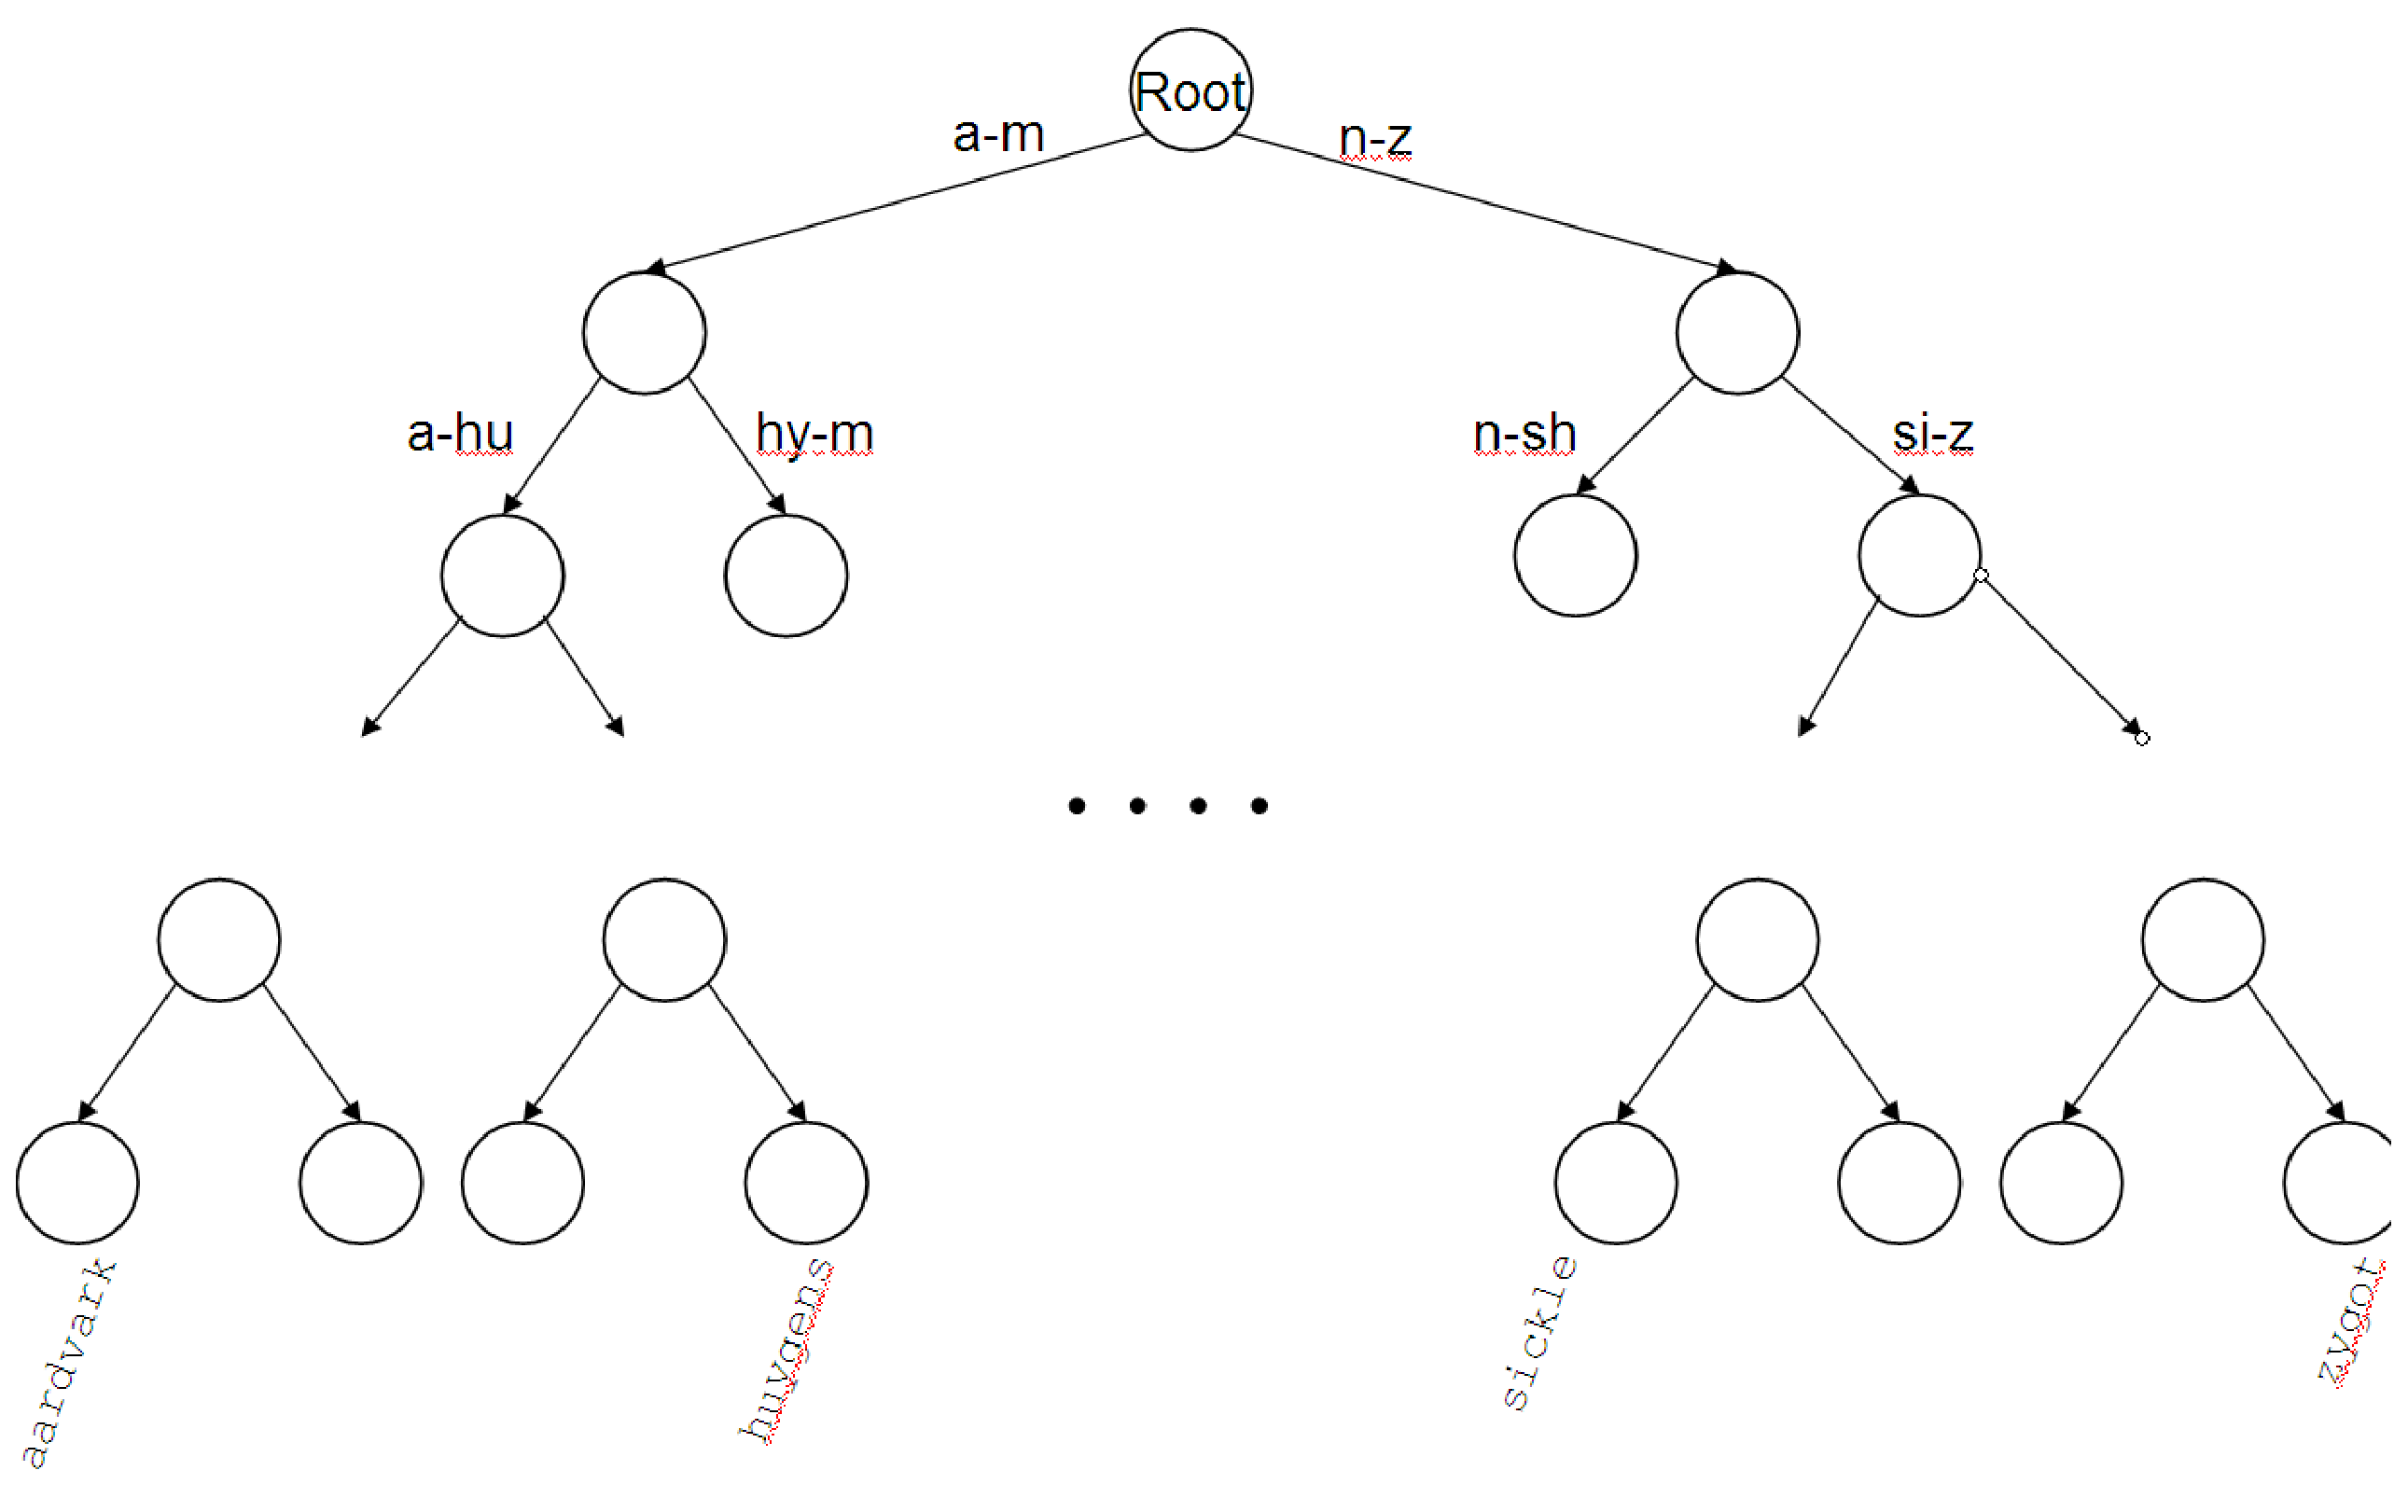
\includegraphics[width=11cm]{bst.eps}
\end{frame}

\begin{frame}
\frametitle{Árvore B}
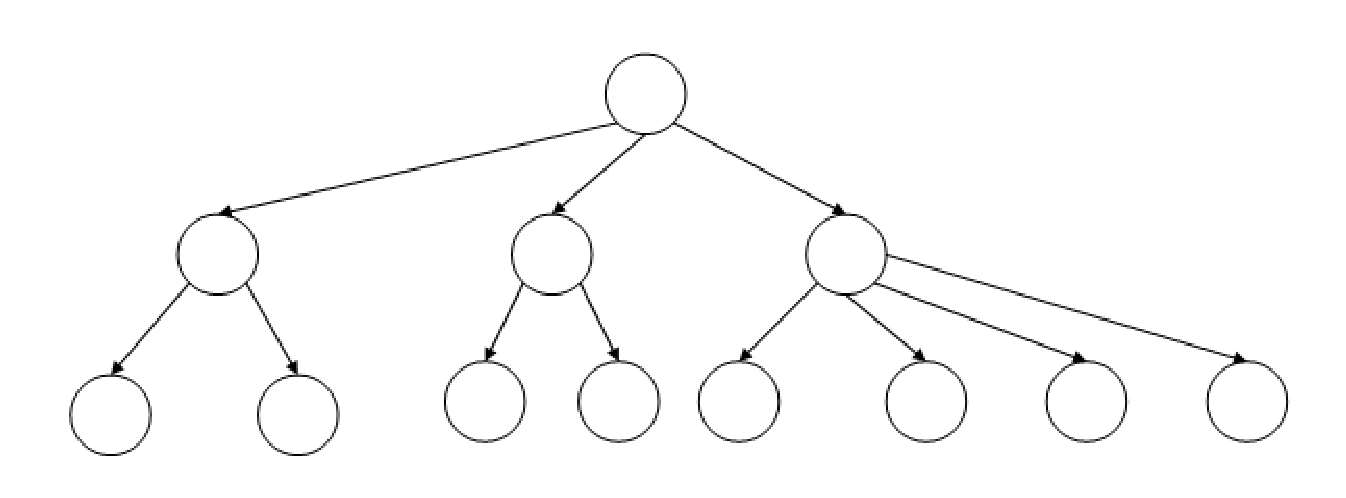
\includegraphics[width=11cm]{btree.eps}
\end{frame}
 
 \section{Consultas Coringa}

\begin{frame}
\frametitle{Consultas coringa}
\begin{itemize}[<+->]
\item \query{mon*}: Encontre todos os documentos contendo termos começados 
por \emph{mon}
\item Fácil com dicionários baseados em árvore B: recupera todos os termos $t$ 
no intervalo: $ \mbox{mon} \leq t < 
%%>
\mbox{moo}$
\item \query{*mon}: Encontre todos os documentos contendo termos que terminam 
com \emph{mon}
\begin{itemize}[<+->]
\item Mantém uma árvore adicional para termos  \emph{ao contrário}
\item Então recupera todos os termos $t$ no intervalo: $
  \mbox{nom} \leq t < 
%%>
\mbox{non}$
\end{itemize}
\item Resultado: Um conjunto de termos que correspondem à consulta 
coringa
\item Então recupera todos os documentos que contenham estes termos
\end{itemize}
\end{frame}

\begin{frame}
\frametitle{Como lidar com um * no meio de um termo}
\begin{itemize}[<+->]
\item Exemplo: \query{m*nchen}
\item Poderíamos buscar todos os termos que satisfazem \query{m*} e
\query{*nchen} Na árvore B e reter a interseção dos dois conjuntos.
\item Mas sai caro
\item Alternativa: índice {\color{blue} permuterm} 
\item Idéia básica: Rotaciona cada consulta coringa, de forma que o * ocorra no 
final.
\item Armazena cada uma destas rotações no dicionário, por exemplo, em uma 
árvore B
\end{itemize}
\end{frame}

\begin{frame}
\frametitle{Índice Permuterm }
\begin{itemize}[<+->]
\item Para o termo \term{hello}: adicione 
\emph{hello\$},
\emph{ello\$h},
\emph{llo\$he},
\emph{lo\$hel}, 
\emph{o\$hell}, e
\emph{\$hello}
  à árvore B onde \$ é um símbolo especial
\end{itemize}
\end{frame}

\begin{frame}
\frametitle{Permuterm $\rightarrow$ mapeamento de termos}
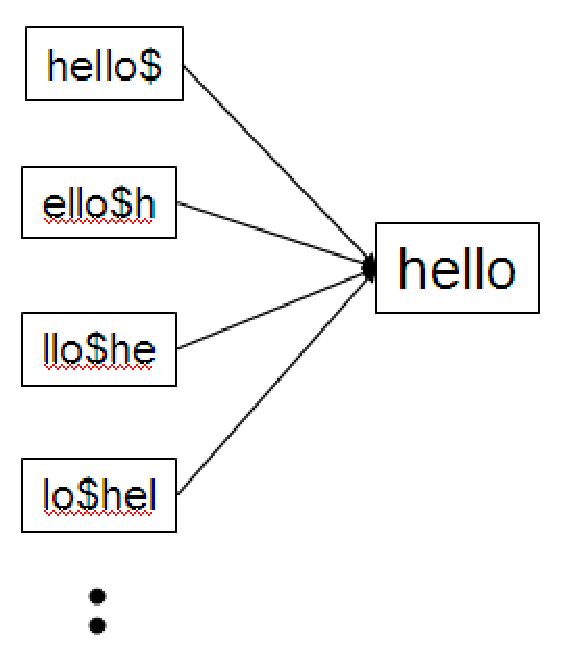
\includegraphics[width=5.5cm]{permuterm.eps}
\end{frame}

\begin{frame}
\frametitle{Índice Permuterm }
\begin{itemize}[<+->]
\item Para \term{hello}, adicionamos:
\emph{hello\$},
\emph{ello\$h},
\emph{llo\$he},
\emph{lo\$hel}, e
\emph{o\$hell}
\item Consultas
\begin{itemize}[<+->]
\item Para X, acesse X\$
\item Para X*, acesse \$X*
\item Para *X, acesse X\$*
\item Para *X*, acesse X*
\item Para X*Y, acesse Y\$X*
\item Example: Para hel*o, acesse o\$hel*
%\item \mygreen{How do we handle X*Y*Z?}
\end{itemize}
\item Um nome mais adequado para um índice Permuterm  seria uma árvore 
permuterm \myblue{tree}.
\item Mas índice permuterm é o nome mais comum.
\end{itemize}
\end{frame}

\begin{frame}
\frametitle{Processando um acesso ao índice permuterm }
\begin{itemize}[<+->]
\item Rotacione a consulta coringa para a direita
\item Use o acesso à árvore B como descrito anteriormente
\item Problema: O Permuterm mais do que {\color{blue} quadruplica} 
o tamanho do dicionário quando comparado a uma árvore B regular. 
(observação empírica)
\end{itemize}
\end{frame}

\section{Distância de Edição}

\begin{frame}[<+->]
\frametitle{Correção ortográfica}
\pause[2]
\begin{itemize}
\item Dois usos principais
\begin{itemize}
\item Correção de documentos a serem indexados
\item Correção de consultas
\end{itemize}
\item Dois métodos diferentes para correção ortográfica
\item Correção de {\color{blue} Palavra isolada} 
\begin{itemize}
\item Verifica cada palavra isoladamente quanto à correção 
ortográfica
\item Não ``pega'' erros que resultam em palavras corretas, p.ex., \emph{an 
asteroid that fell {\color{blue} form} the sky}
\end{itemize}
\item Correção ortográfica {\color{blue} contextual} 
\begin{itemize}
\item Olha para as palavras vizinhas
\item Pode corrigir o erro \emph{form}/\emph{from} acima
\end{itemize}
\end{itemize}
\end{frame}

\begin{frame}[<+->]
\frametitle{Corrigindo documentos}
\pause[2]
\begin{itemize}
\item Não estamos interessados em correção interativa de documentos
(p.ex., MS Word) neste curso.
\item Em RI, Usamos a correção de documentos primariamente para documentos 
OCR-izados. (OCR = optical character recognition)
\item A filosofia geral em RI é: Não altere os documentos.
\end{itemize}
\end{frame}

\begin{frame}[<+->]
\frametitle{Corrigindo consultas}
\pause[2]
\begin{itemize}
\item Primeiro: correção ortográfica de palavras isoladas
\item Premissa 1: Há uma lista de palavas ``corretas'' a partir da qual as 
correções podem ser obtidas.
\item Premissa 2: Há uma maneira de calcular a {\color{blue} distância} entre 
uma palavra errada e uma correta.
\item Algoritmo simplificado: retorne a palavra ``correta'' com a menor 
distância da palavra errada.
\item Exemplo: \emph{informaton} $\rightarrow$ \emph{information}
\item Como lista de palavras corretas, podemos usar o vocabulário de todas as 
palavras que ocorrem em nossa coleção.
\item {\color{green} Porque isto é problemático?} 
\end{itemize}
\end{frame}

\begin{frame}[<+->]
\frametitle{Alternativas  ao uso do vocabulário de termos}
\pause[2]
\begin{itemize}
\item Um dicionário padrão (Webster's, Aurélio etc.)
\item Um dicionário de um domínio específico (Para sistemas de RI 
especializados)
\item O vocabulário de termos ponderado, ponderado de forma 
adequada
\end{itemize}
\end{frame}

\begin{frame}[<+->]
\frametitle{Distância entre a palavra errada e a ``correta''}
\pause[2]
\begin{itemize}
\item Estudaremos várias alternativas.
\item Distância de edição e a distância de Levenshtein 
\item Distância de edição ponderada
\item sobreposição de $k$-grams
\end{itemize}
\end{frame}

\begin{frame}[<+->]
\frametitle{Distância de edição}
\pause[2]
\begin{itemize}
\item A distância de edição entre a string $s_1$ e a string $s_2$ é o número 
mínimo de operações básicas que converte $s_1$ em
$s_2$.
\item Distância de Levenshtein: Operações válidas: inserção, deleção, e
substituição
\item Distância de Levenshtein \emph{dog}-\emph{do}: 1
\item Distância de Levenshtein \emph{cat}-\emph{cart}: 1
\item Distância de Levenshtein \emph{cat}-\emph{cut}: 1
\item Distância de Levenshtein \emph{cat}-\emph{act}: 2
\item Distância de Damerau-Levenshtein \emph{cat}-\emph{act}: 1
\item Distância de Damerau-Levenshtein inclui a transposição como uma quarta 
operação possivel.
\end{itemize}
\end{frame}


\begin{frame}
\frametitle{Distância de Levenshtein: Computação}

\bigskip

\begin{tabular}{ ||c ||c ||c ||c ||c ||c ||}\hline\hline
& & f & a & s & t \\\hline\hline
& 

 0& 1&2&3&4\\\hline\hline
c & 1&1&2&3&4\\\hline\hline
a & 2&2&1&2&3\\\hline\hline
t & 3&3&2&2&2\\\hline\hline
s & 4&4&3&2&3\\\hline\hline
\end{tabular}

\end{frame}


\begin{frame}
\frametitle{Distância de Levenshtein: Algoritmo}

\begin{algorithm}{LevenshteinDistance}{s_1,s_2}
\begin{FOR}
{i \= 0 \TO |s_1|}
m[i,0] = i
\end{FOR}\\
\begin{FOR}
{j \= 0 \TO |s_2|}
m[0,j] = j
\end{FOR}\\
\begin{FOR}
{i \= 1 \TO |s_1|}
\begin{FOR}
{j \= 1 \TO |s_2|}
\begin{IF}{s_1[i]=s_2[j]}
m[i,j] = \min\{m[i\mbox{-}1, j] \mbox{+} 1,m[i, j\mbox{-}1] \mbox{+} 
1,m[i\mbox{-}1,j\mbox{-}1] \}
\ELSE
m[i,j] = \min\{m[i\mbox{-}1, j] \mbox{+} 1,m[i, j\mbox{-}1] \mbox{+} 
1,m[i\mbox{-}1,j\mbox{-}1]\mbox{+}1 \}
\end{IF}
\end{FOR}
\end{FOR}\\
\RETURN{m[|s_1|,|s_2|]}
\end{algorithm}

Operações: inserção (custo 1), deleção (custo 1), substituição (custo
1), cópia (custo 0)

\end{frame}

\begin{frame}
\frametitle{Distância de Levenshtein: Algoritmo}

\begin{algorithm}{LevenshteinDistance}{s_1,s_2}
\begin{FOR}
{i \= 0 \TO |s_1|}
m[i,0] = i
\end{FOR}\\
\begin{FOR}
{j \= 0 \TO |s_2|}
m[0,j] = j
\end{FOR}\\
\begin{FOR}
{i \= 1 \TO |s_1|}
\begin{FOR}
{j \= 1 \TO |s_2|}
\begin{IF}{s_1[i]=s_2[j]}
m[i,j] = \min\{m[i\mbox{-}1, j] \mbox{+} 1, \myred{m[i, j\mbox{-}1] \mbox{+} 
1},m[i\mbox{-}1,j\mbox{-}1] \}
\ELSE
m[i,j] = \min\{m[i\mbox{-}1, j] \mbox{+} 1, \myred{m[i, j\mbox{-}1] \mbox{+} 
1},m[i\mbox{-}1,j\mbox{-}1]\mbox{+}1 \}
\end{IF}
\end{FOR}
\end{FOR}\\
\RETURN{m[|s_1|,|s_2|]}
\end{algorithm}

Operações: {\color{red} inserção (custo 1)}, deleção (custo 1), substituição 
(custo
1), cópia (custo 0)


\end{frame}

\begin{frame}
\frametitle{Distância de Levenshtein: Algoritmo}

\begin{algorithm}{LevenshteinDistance}{s_1,s_2}
\begin{FOR}
{i \= 0 \TO |s_1|}
m[i,0] = i
\end{FOR}\\
\begin{FOR}
{j \= 0 \TO |s_2|}
m[0,j] = j
\end{FOR}\\
\begin{FOR}
{i \= 1 \TO |s_1|}
\begin{FOR}
{j \= 1 \TO |s_2|}
\begin{IF}{s_1[i]=s_2[j]}
m[i,j] = \min\{ \myred{m[i\mbox{-}1, j] \mbox{+} 1},m[i, j\mbox{-}1] \mbox{+} 
1,m[i\mbox{-}1,j\mbox{-}1] \}
\ELSE
m[i,j] = \min\{ \myred{m[i\mbox{-}1, j] \mbox{+} 1},m[i, j\mbox{-}1] \mbox{+} 
1,m[i\mbox{-}1,j\mbox{-}1]\mbox{+}1 \}
\end{IF}
\end{FOR}
\end{FOR}\\
\RETURN{m[|s_1|,|s_2|]}
\end{algorithm}


Operações: inserção (custo 1), {\color{red} deleção (custo 1)}, substituição 
(custo
1), cópia (custo 0)

\end{frame}

\begin{frame}
\frametitle{Distância de Levenshtein: Algorithm}

\begin{algorithm}{LevenshteinDistance}{s_1,s_2}
\begin{FOR}
{i \= 0 \TO |s_1|}
m[i,0] = i
\end{FOR}\\
\begin{FOR}
{j \= 0 \TO |s_2|}
m[0,j] = j
\end{FOR}\\
\begin{FOR}
{i \= 1 \TO |s_1|}
\begin{FOR}
{j \= 1 \TO |s_2|}
\begin{IF}{s_1[i]=s_2[j]}
m[i,j] = \min\{m[i\mbox{-}1, j] \mbox{+} 1,m[i, j\mbox{-}1] \mbox{+} 
1,m[i\mbox{-}1,j\mbox{-}1] \}
\ELSE
m[i,j] = \min\{m[i\mbox{-}1, j] \mbox{+} 1,m[i, j\mbox{-}1] \mbox{+} 1, 
\myred{m[i\mbox{-}1,j\mbox{-}1]\mbox{+}1} \}
\end{IF}
\end{FOR}
\end{FOR}\\
\RETURN{m[|s_1|,|s_2|]}
\end{algorithm}

Operações: inserção (custo 1), deleção (custo 1), {\color{red} substituição 
(custo
1)}, cópia (custo 0)


\end{frame}

\begin{frame}
\frametitle{Distância de Levenshtein: Algoritmo}

\begin{algorithm}{LevenshteinDistance}{s_1,s_2}
\begin{FOR}
{i \= 0 \TO |s_1|}
m[i,0] = i
\end{FOR}\\
\begin{FOR}
{j \= 0 \TO |s_2|}
m[0,j] = j
\end{FOR}\\
\begin{FOR}
{i \= 1 \TO |s_1|}
\begin{FOR}
{j \= 1 \TO |s_2|}
\begin{IF}{s_1[i]=s_2[j]}
m[i,j] = \min\{m[i\mbox{-}1, j] \mbox{+} 1,m[i, j\mbox{-}1] \mbox{+} 1, 
\myred{m[i\mbox{-}1,j\mbox{-}1]} \}
\ELSE
m[i,j] = \min\{m[i\mbox{-}1, j] \mbox{+} 1,m[i, j\mbox{-}1] \mbox{+} 
1,m[i\mbox{-}1,j\mbox{-}1]\mbox{+}1 \}
\end{IF}
\end{FOR}
\end{FOR}\\
\RETURN{m[|s_1|,|s_2|]}
\end{algorithm}

Operações: inserção (custo 1), deleção (custo 1), substituição (custo
1), {\color{red} cópia (custo 0)}


\end{frame}

\begin{frame}[label=lmatrix]
\frametitle{Distância de Levenshtein: Exemplo}

\bigskip

\begin{tabular}{ ||c ||c ||c ||c ||c ||c ||}\hline\hline
& & f & a & s & t \\\hline\hline
& \begin{tabular}{l|l}&\\\hline&{\bf 0}\end{tabular} &
\begin{tabular}{l|l}&\\\hline{\bf 1 }&{\bf 1 }\end{tabular} &
\begin{tabular}{l|l}&\\\hline{\bf 2 }&{\bf 2 }\end{tabular} &
\begin{tabular}{l|l}&\\\hline{\bf 3 }&{\bf 3 }\end{tabular} &
\begin{tabular}{l|l}&\\\hline{\bf 4 }&{\bf 4 }\end{tabular} \\\hline\hline
c & \begin{tabular}{l|l}&{\bf 1 }\\\hline&{\bf 1 }\end{tabular}
&
\begin{tabular}{l|l} \textsl{{1}} & \textsl{2} \\\hline \textsl{2} & 
\textsl{{1}} \end{tabular} & \begin{tabular}{l|l} {\bf 2} & 3 \\\hline {\bf 2} & 
{\bf 2} \end{tabular} & \begin{tabular}{l|l} {\bf 3} & 4 \\\hline {\bf 3} & {\bf 
3} \end{tabular} & \begin{tabular}{l|l} {\bf 4} & 5 \\\hline {\bf 4} & {\bf 4} 
\end{tabular} \\\hline\hline
a & \begin{tabular}{l|l}&{\bf 2 }\\\hline&{\bf 2 }\end{tabular}
& \begin{tabular}{l|l} {\bf 2} & {\bf 2} \\\hline 3 & {\bf 2} \end{tabular} &
\begin{tabular}{l|l} \textsl{{1}} & \textsl{3} \\\hline \textsl{3} & 
\textsl{{1}} \end{tabular}  &
\begin{tabular}{l|l} \textsl{3} & \textsl{4} \\\hline \textsl{{2}} & 
\textsl{{2}} \end{tabular} & \begin{tabular}{l|l} 4 & 5 \\\hline {\bf 3} & {\bf 
3} \end{tabular} \\\hline\hline
t & \begin{tabular}{l|l}&{\bf 3 }\\\hline&{\bf 3 }\end{tabular}
& \begin{tabular}{l|l} {\bf 3} & {\bf 3} \\\hline 4 & {\bf 3} \end{tabular} & 
\begin{tabular}{l|l} 3 & {\bf 2} \\\hline 4 & {\bf 2} \end{tabular} & 
\begin{tabular}{l|l} {\textsl{2}} & \textsl{3} \\\hline \textsl{3} & 
{\textsl{2}} \end{tabular} &
\begin{tabular}{l|l} \textsl{{2}} & \textsl{4} \\\hline \textsl{3} & 
\textsl{{2}} \end{tabular} \\\hline\hline
s & \begin{tabular}{l|l}&{\bf 4 }\\\hline&{\bf 4 }\end{tabular}
& \begin{tabular}{l|l} {\bf 4} & {\bf 4} \\\hline 5 & {\bf 4} \end{tabular} & 
\begin{tabular}{l|l} 4 & {\bf 3} \\\hline 5 & {\bf 3} \end{tabular} & 
\begin{tabular}{l|l} {\bf 2} & 3 \\\hline 4 & {\bf 2} \end{tabular} &
\begin{tabular}{l|l} \textsl{{3}} & \textsl{{3}} \\\hline \textsl{{3}} & 
\textsl{{3}} \end{tabular} \\\hline\hline
\end{tabular}

\end{frame}

\begin{frame}
\frametitle{Cada célula da matriz de Levenshtein}

\bigskip

\begin{tabular}{|l|l|}

\hline
\parbox{4cm}{Custo de chegar aqui a partir do meu vizinho superior 
esquerdo (cópia or substituição)} &
\parbox{4cm}{Custo de chegar aqui a partir do meu vizinho superior 
(deleção)}\\\hline
\parbox{4cm}{Custo de chegar aqui a partir do meu vizinho esquerdo (inserção)} &
\parbox{4cm}{mínimo dos três ``movimentos'' possíveis; a forma mais barata de 
chegar aqui
} \\\hline

\end{tabular}

\end{frame}

\againframe<2>{lmatrix}

\end{document}
